\chapter{Anforderungsanalyse}

In der hier durchzuführenden Analyse soll ein neues Konzept für das Bestell- und Verwaltungssystem dargestellt werden. Auf der Basis der IST-Analyse wird eine Verbesserung mit aktuellen Webtechnologie und Verfahren durchgeführt. In diesem Kapitel sollen die bestehenden Probleme und das Optimierungspotenzial näher betrachtet werden.
Das neue Bestellsystem soll nicht kompliziert sein, sondern benutzerfreundlich. Die Optionen sollen deutlich zu erkennen und einfach zu bedienen sein. Sicherheit ist ein wesentlicher Teil der webbasierten Entwicklung, weshalb zusätzliche Prüfungen in dieser Richtung eingeführt werden. Die Auftragsverwaltung und die Kundenübersicht werden ihre behalten. Das gesamte Konzept wird aus einer Umbraco-Instanz heraus verwaltet. Im folgenden Unterkapitel werden die oben beschriebenen Anforderungen erweitert und erläutert.



\section{Paket A}

Die aktuelle Software gibt dem Auftraggeber wenige Möglichkeiten, Änderungen im Frontend vorzunehmen. Es wurde immer ein Entwickler benötigt, um etwas zu ändern. Beispielsweise kann der Auftraggeber nicht einmal die Schrift oder die Farbe des Textes editieren.
In diesem Unterkapitel wird versucht, dem Auftraggeber in diesem Bereich völlige Freiheit zu lassen. Es wird besonders darauf geachtet, dass die Möglichkeiten, zu ändern und editieren, erhalten bleiben. Als Beispiele wurden Schriftart und Farbe vorgegeben.
Dazu wird die Verwendung von Grids, Makros und Formularen empfohlen. Diese und weitere Begriffe werden im nächsten Kapitel erläutert.

\section{Paket B}


\subsection{Kundenverwaltung}

In diesem Unterkapitel werden die Anforderungen betrachtet, die der Auftraggeber gestellt hat, um die Kundenaktivitäten besser kontrollieren zu können. Es wird eine eigene Seite für ihn erstellt, in der Kunden Bestellungen erstellen und einsehen oder Nachrichten verschicken oder lesen können.

\subsubsection{Kundenerfassung}

Hier werden die Anforderungen zum Onlinebestellsystem und der Kundenübersicht beschrieben.

\begin{enumerate}
	\item 1.	Der Kunde kann sich bei der Erstbestellung registrieren und erhält per E-Mail eine PIN. Bei jeder weiteren Bestellung kann er sich mit seiner E-Mail und der PIN einloggen. Es soll darauf geachtet werden, dass beim Bestellen die E-Mail-Adresse überprüft werden muss. Wenn die eingegebene E-Mail-Adresse bereits verwendet wurde, soll ein Hinweis erscheinen. Für Neukunden steht eine private Profil-Seite zur Verfügung. Nach der Registrierung ist es möglich, dass der Kunde eine erste Bestellung tätigt, für weitere Anmeldungen muss er jedoch vom Auftraggeber bestätigt werden. Nach dieser Bestätigung erhält der Kunde bereits erwähnte PIN. In den Abbildungen \ref{fig:registerForm} und \ref{fig:anmeldeformular} sind das Register- und das Anmeldeformular zu sehen. Nach den vorgegebenen Anforderungen sind zu diesem Punkt die Funktionalitäten nicht zu ändern. In die Entwicklung müssen die bereits erläuterten Funktionalitäten und Aktivitäten in der Umbraco implementiert werden.
	
\end{enumerate} 

\subsubsection{Kundenansicht}

\begin{enumerate}
	\item Wenn der Kunde vom Auftraggeber verifiziert wird, kann er sich mit seiner E-Mail und seiner PIN einloggen und seine aktuelle Bestellung wie auch die vergangenen Bestellungen einsehen. Für Kommunikation und Absprachen wird ein Kontaktfenster verwendet. Der Auftraggeber kann entweder allgemeine Information an seine Kunden schicken oder kundenspezifisch antworten. Die Abbildung \ref{fig:KundenAnsicht} stellt die bisherige Kundenansicht mit den alten Funktionalitäten dar. Diese sollen nicht geändert, sondern in dem neuen System implementiert werden. Die Kunden sollen über die Member-Section im Umbraco integriert werden.
	
\end{enumerate} 

\subsubsection{Auftraggeber-Ansicht}

\begin{enumerate}
\item Der Auftraggeber erhält eine Kundenübersicht, die er filtern kann. In der Detailansicht sieht er die Informationen über Kunden. Dort kann er den Bestellverlauf nachverfolgen und aus der Ansicht heraus E-Mails an den Kunden senden (Mail-Vorlage oder frei gestaltbar). Dies wird in den Abbildungen \ref{fig:KundenDatei} und \ref{fig:KundenEditor} dargestellt. In dem neuen Konzept wird gefordert, dass die Funktionalitäten der alten Software im neuen System gleich bleiben.
\end{enumerate} 

\subsubsection{Kommunikation}

\begin{enumerate}
	\item Über die Option „neue Nachrichten“ kann der Auftraggeber mit seinen Kunden kommunizieren und Absprachen zu den Aufträgen treffen.
	\item Für das neuen Konzept soll eine neue Kommunikationsmethode für die alte Funktionalitäten mit Filtern (z. B. gelesen und nach Kunden) integriert werden. Der „Chat“ sollte aus der Kundenkartei-Ansicht ebenfalls funktionieren und die Kommunikation soll an einen Auftrag gebunden sein. 
	Die Kommunikationsübersicht wird in Abbildung \ref{fig:NachrichtErscheint} illustriert. 
	\begin{figure}[h]
		\centering
		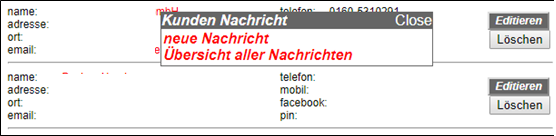
\includegraphics[width=0.7\linewidth]{Graphics/newNach.png}
		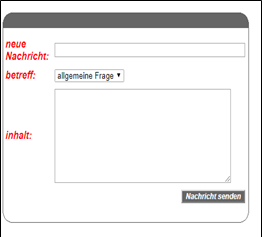
\includegraphics[width=0.7\linewidth]{Graphics/newNachr.png}
		\caption[Neue Nachricht]{Die bisherige Eingabemaske für die Nachricht}
		\label{fig:NachrichtErscheint}
	\end{figure}

\end{enumerate} 
Im neuen System soll dasselbe Funktionalität des Chats bleiben.

\subsection{Artikelverwaltung}

\subsubsection{Artikel erfassen, ändern und löschen}

\begin{enumerate}
	\item Der Auftraggeber kann in einer recht einfachen Maske Artikel verwalten (online-editor). Es gibt nur zwei Kategorien: Arrangements und Artikel-Standard. Derzeit sind die Arrangements noch nicht mit den Webseiten gekoppelt, aber sie müssen in der neuen Software daran gebunden werden.
	\item Ein Arrangement besteht aus Kategorien (fest vorgegeben) und Positionen und kann sich darin unterscheiden, ob Kunden Positionen auswählen dürfen oder nicht.
	\item Es wird gefordert, dass die Artikel einfacher verwaltet werden können und die Artikelseite der Webseite direkt mit dem Artikel gekoppelt sein soll.
	
	Die Bisherige Übersicht zum Artikel ist in den Abbildungen \ref{fig: Online-EditorUebersicht} und \ref{fig: Editor-Menü2} zu sehen.
	
\end{enumerate} 


\subsection{Auftragsverwaltung}

\subsubsection{Übersicht}

\begin{enumerate}
	\item Der Auftraggeber erhält eine Übersicht über seine aktuellen Aufträge. Für jede Art von Auftrag (neu, bearbeitet, vergangen und fällig) gibt es einen Select-Befehl.
	\item Diese Ansicht soll in einer eigenen Umbraco-Subsection umgesetzt werden. Die Artikeldatenbank soll von Access nach SQL transportiert werden. Es muss eine neue Zuordnung von Kunde zu Umbraco-Member geben. In der Abbildung \ref{fig:Uebersicht} ist die Übersicht zu sehen.
	
	\begin{figure}[h]
		\centering
		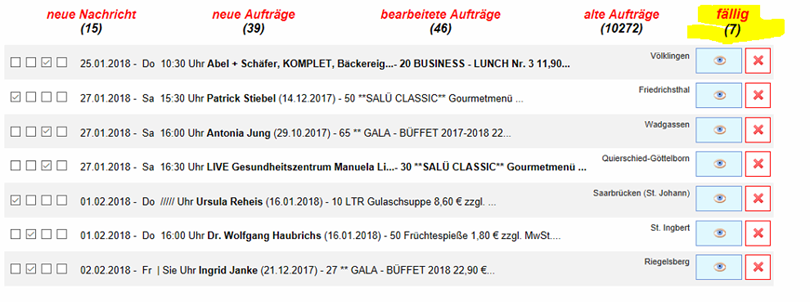
\includegraphics[width=0.7\linewidth]{Graphics/Uebersicht.png}
		\caption[Uebersicht]{Die bisherige Eingabemaske für die Übersicht}
		\label{fig:Uebersicht}
	\end{figure}
\end{enumerate} 



\subsubsection{Detailansicht}

\begin{enumerate}
	\item In der Detailansicht kann der Auftraggeber den Auftrag bearbeiten, den Status ändern, Positionen editieren, hinzufügen und löschen, dem Kunden Freigaben erteilen (z. B. Aussuchen der Positionen) und eine Rechnungsnummer vergeben.
	\item Der Auftrag muss auf vier Seiten ausdruckbar (genau vorgegeben) sein.
	\item Die Daten der Auftraggeber und der Kunden von zweitem Blatt müssen für Auftraggeber zur Verfügung stehen, damit er sie selbst ändern kann.
	\item Quick-Icons erleichtern die Kommunikation mit dem Kunden und die Anpassung an dessen Auswahl zu Auftragsbeginn (z.B. Änderung Serviceauswahl).
	\item  Diese Ansicht soll in einer eigenen Umbraco-subsection umgesetzt werden.
	
	Detailansicht wird in der Abbildung \ref{fig:Detailansicht} dargestellt.
	\begin{figure}[h]
		\centering
		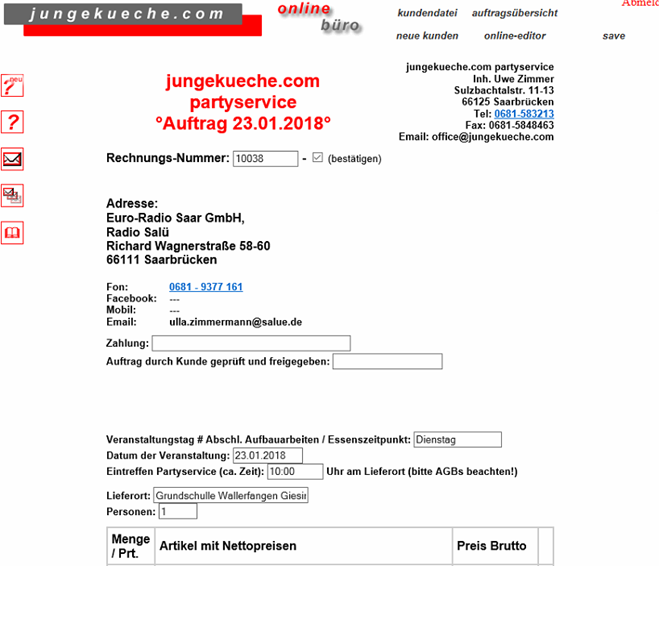
\includegraphics[width=0.7\linewidth]{Graphics/detailansichtt.png}
		\caption[Detailansicht]{Die bisherige Eingabemaske für die Detailansicht}
		\label{fig:Detailansicht}
	\end{figure}
\end{enumerate} 


\subsection{E-Mail-Verwaltung}

\begin{enumerate}
	\item Hier kann der Auftraggeber E-Mail Vorlagen mit Platzhaltern definieren, die er dann in der Kundenkommunikation auswählen kann.
	\item Es gibt ein Formular für Terminanfragen über die Webseite. Diese erzeugt eine E-Mail an den Auftraggeber, der in der E-Mail nur einen Link betätigen muss, um die Anfrage zu bestätigen. Dies hängt auch mit dem E-Mail Verwaltungssystem zusammen.
	\item Diese Ansicht soll in einer eigenen Umbraco-subsection umgesetzt werden.
	Siehe dazu Abbildung \ref{fig:email}.
	
	\begin{figure}[h]
	\centering
	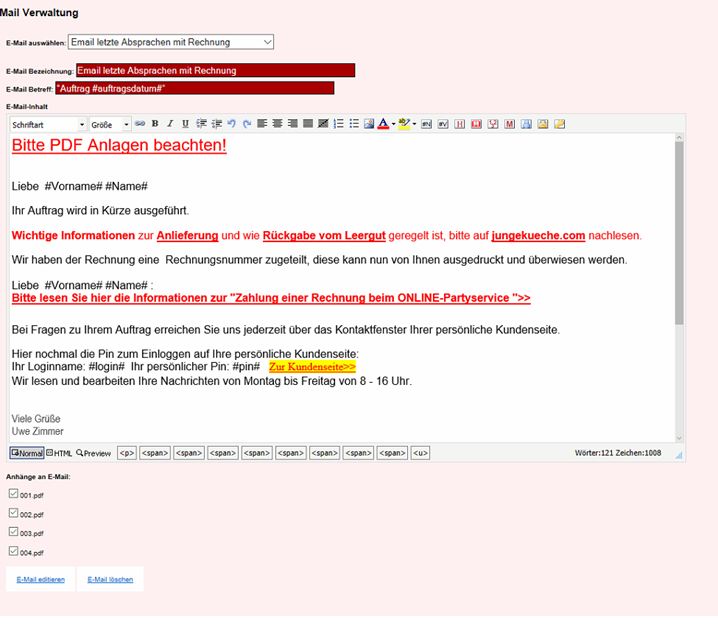
\includegraphics[width=0.5\linewidth]{Graphics/email.png}
	\caption[E-Mail-Verwaltung]{Die bisherige Eingabemaske für die E-Mail-Verwaltung}
	\label{fig:email}
\end{figure}
\end{enumerate} 



\subsection{Umsatzverfassung}
\begin{enumerate}
	\item Hier kann der Auftraggeber die Umsätze der letzten Monate / Jahre, die über die Aufträge zustande gekommen sind, einsehen. Dabei ist es wichtig, dass diese Datensätze nicht direkt an die Aufträge gekoppelt sind, sondern aus einer separaten Tabelle kommen, die der Auftraggeber auch selbst noch editieren kann.
	\item Diese Ansicht soll in einer eigenen Umbraco-Subsection umgesetzt werden.
	In der Abbildung \ref{fig:Umsatzerfassung} wird die Umsatzerfassung dargestellt.
	
		\begin{figure}[h]
		\centering
		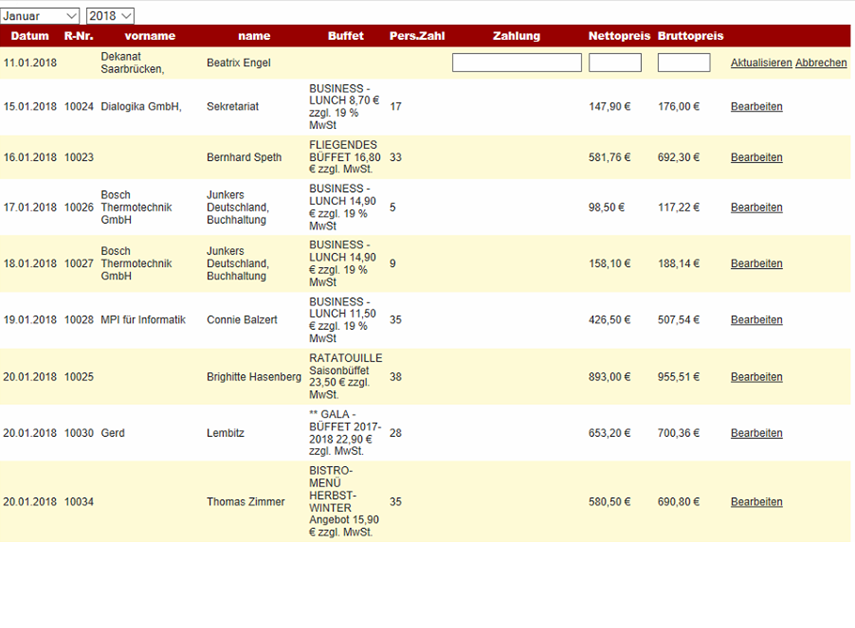
\includegraphics[width=0.6\linewidth]{Graphics/umsatzErfassung.png}
		\caption[Uebersicht]{Die bisherige Eingabemaske für die Umsatzerfassung}
		\label{fig:Umsatzerfassung}
	\end{figure}
	
\end{enumerate} 


